%%%%%%%%%%%%%%%%%%%%%%%%%%%%%%%%%%%%%%%%%%%%%%%%%%%%%%%%%%%%%%%%%%%%%%%%%%%%%%%%%%
\begin{frame}[fragile]\frametitle{}
\begin{center}
{\Large Introduction to Scikit-Learn aka Sklearn}
\end{center}
\end{frame}


%%%%%%%%%%%%%%%%%%%%%%%%%%%%%%%%%%%%%%%%%%%%%%%%%%%%%%%%%%
\begin{frame}[fragile]\frametitle{scikit.learn}

\begin{itemize}
\item Open source machine learning library for Python. 
\item Features various classification, regression and clustering algorithms
% \item Designed to inter-operate with the Python numerical and scientific libraries NumPy and SciPy.
\end{itemize}
\begin{center}

\includegraphics[width=0.6\linewidth,keepaspectratio]{SKL-logo2}
\end{center}
\end{frame}

%%%%%%%%%%%%%%%%%%%%%%%%%%%%%%%%%%%%%%%%%%%%%%%%%%%%%%%%%%
\begin{frame}[fragile]\frametitle{Machine Learning in Python}
\begin{center}
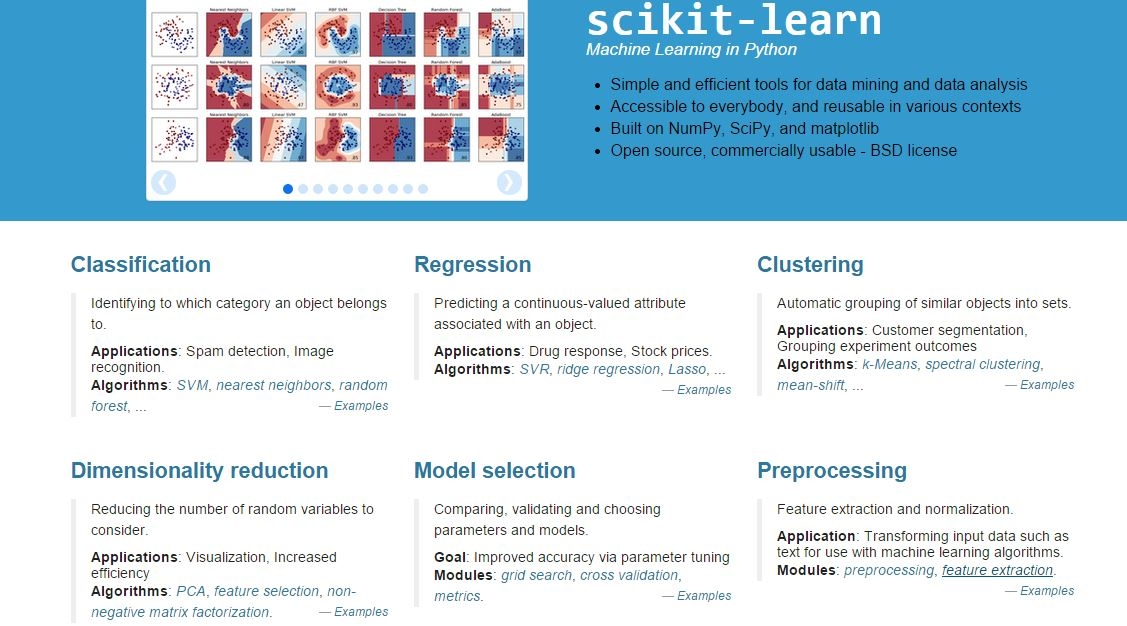
\includegraphics[width=\linewidth,keepaspectratio]{SKLsite}
\end{center}
\end{frame}


%%%%%%%%%%%%%%%%%%%%%%%%%%%%%%%%%%%%%%%%%%%%%%%%%%%%%%%%%%%
%\begin{frame}[fragile]\frametitle{Sci-Kit Learn Site info}
%\begin{center}
%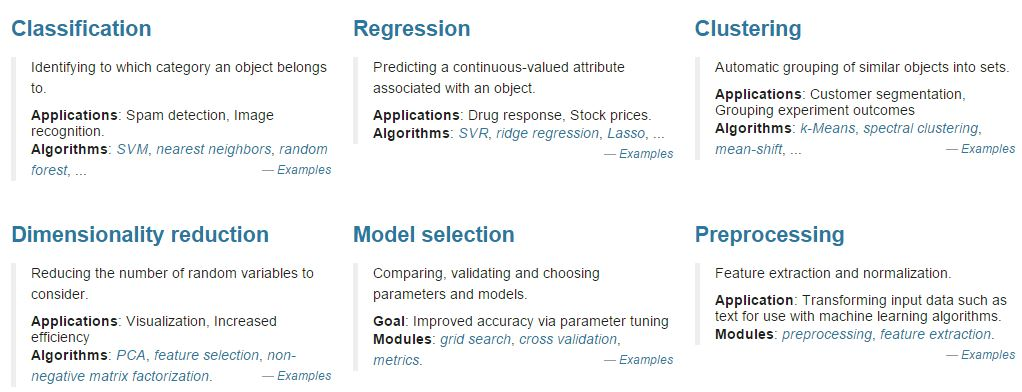
\includegraphics[width=\linewidth,keepaspectratio]{SKLsiteinfo}
%\end{center}
%\end{frame}


%
%%%%%%%%%%%%%%%%%%%%%%%%%%%%%%%%%%%%%%%%%%%%%%%%%%%%%%%%%%%%%%%%%%%%%%%%%
%\begin{frame}[fragile]\frametitle{Scikit-learn}
%\begin{itemize}
%\item Scikit-learn is a library that provides a variety of both supervised and unsupervised machine learning techniques. 
%\item Supervised machine learning refers to the problem of inferring a function from labeled training data, and it comprises both regression and classification. 
%\item	Unsupervised machine learning, on the other hand, refers to the problem of finding interesting patterns or structure in the data; it comprises techniques such as clustering and dimensionality reduction.
%\item  In addition to statistical learning techniques, scikit-learn provides utilities for common tasks such as model selection, feature extraction, and feature selection.
%\end{itemize}
%\end{frame}



%%%%%%%%%%%%%%%%%%%%%%%%%%%%%%%%%%%%%%%%%%%%%%%%%%%%%%%%%%%%%%%%%%%%%%%%
\begin{frame}[fragile]\frametitle{Sklearn Paradigm}
Scikit-learn provides an object-oriented interface centered around the concept of an Estimator.

\end{frame}

%%%%%%%%%%%%%%%%%%%%%%%%%%%%%%%%%%%%%%%%%%%%%%%%%%%%%%%%%%%%%%%%%%%%%%%%
\begin{frame}[fragile]\frametitle{Scikit-Learn's Estimator API}
The steps in using the Scikit-Learn estimator API are as follows
\begin{itemize}
\item Choose a class of model by importing the appropriate estimator class from Scikit-Learn.
\item Choose model hyper-parameters by instantiating this class.
\item Arrange data into a features matrix and target vector.
\item Fit the model to your data by calling the fit() method of the model instance.
\begin{itemize}
    \item For supervised learning, predict labels for unknown data using the predict().
    \item For unsupervised learning, transform or infer properties of the data using transform() or predict().
\end{itemize}
\end{itemize}
\end{frame}

%%%%%%%%%%%%%%%%%%%%%%%%%%%%%%%%%%%%%%%%%%%%%%%%%%%%%%%%%%%%%%%%%%%%%%%%
\begin{frame}[fragile]\frametitle{}
\begin{itemize}
\item The \texttt{Estimator.fit} method sets the state of the estimator based on the training data. 
\item Usually, the data is comprised of a two-dimensional numpy array X of shape \texttt{(n\_samples, n\_predictors) }that holds the so-called feature matrix and a one-dimensional numpy array y that holds the responses. 
\item Some estimators allow the user to control the fitting behavior. 
\end{itemize}
\end{frame}

%%%%%%%%%%%%%%%%%%%%%%%%%%%%%%%%%%%%%%%%%%%%%%%%%%%%%%%%%%
\begin{frame}[fragile]\frametitle{Estimator}
\begin{lstlisting}
class Estimator(object):
    def fit(self, X, y=None):
        """Fits estimator to data. """
        # set state of ''self''
        return self
    def predict(self, X):
        """Predict response of ''X''. """
        # compute predictions ''pred''
        return pred
\end{lstlisting}
\begin{itemize}
\item fit(X,y) sets the state of the estimator.
\item  X is usually a 2D numpy array of shape (num\_samples, num\_features).
\item  y is a 1D array with shape (n\_samples,)
\item  predict(X) returns the class or value
%\item  predict\_proba() returns a 2D array of shape (n\_samples, n\_classes)
\end{itemize}
\end{frame}

%%%%%%%%%%%%%%%%%%%%%%%%%%%%%%%%%%%%%%%%%%%%%%%%%%%%%%%%%%%%%%%%%%%%%%%%%%%%%%%%%%
\begin{frame}[fragile]\frametitle{}
\begin{center}
{\Large Sklearn: Installations}
\end{center}
\end{frame}

%%%%%%%%%%%%%%%%%%%%%%%%%%%%%%%%%%%%%%%%%%%%%%%%%%%%%%%%%%%
%\begin{frame}[fragile]\frametitle{}
%
%\begin{center}
%We will introduce the basic categories of learning problems and how to implement them using scikit-learn.
%\end{center}
%\end{frame}




%%%%%%%%%%%%%%%%%%%%%%%%%%%%%%%%%%%%%%%%%%%%%%%%%%%%%%%%%%%
\begin{frame}[fragile]\frametitle{Scikit Learn:  Installation and setup}
Install Anaconda distribution having Python 3.5
% \begin{itemize}
% \item 	Python version 2.6-2.7 or 3.3-3.4
% \item     numpy version 1.5 or later: http://www.numpy.org/
% \item     scipy version 0.10 or later: http://www.scipy.org/
% \item     matplotlib version 1.3 or later: http://matplotlib.org/
% \item     scikit-learn version 0.14 or later: http://scikit-learn.org
% %\item     ipython version 2.0 or later, with notebook support: http://ipython.org
% % \item     seaborn: version 0.5 or later, used mainly for plot styling
% \end{itemize}
\lstinline|$ conda install numpy scipy matplotlib scikit-learn ipython-notebook|
\end{frame}

%%%%%%%%%%%%%%%%%%%%%%%%%%%%%%%%%%%%%%%%%%%%%%%%%%%%%%%%%%%
\begin{frame}[fragile]\frametitle{Checking your installation}
\begin{lstlisting}
import numpy
print('numpy:', numpy.__version__)

import scipy
print('scipy:', scipy.__version__)

import matplotlib
print('matplotlib:', matplotlib.__version__)

import sklearn
print('scikit-learn:', sklearn.__version__)

import seaborn
print('seaborn', seaborn.__version__)
\end{lstlisting}
\end{frame}

%
%%%%%%%%%%%%%%%%%%%%%%%%%%%%%%%%%%%%%%%%%%%%%%%%%%%%%%%%%%%%%%%%%%%%%%%%%
%\begin{frame}[fragile]\frametitle{Loading the Iris Data with Scikit-Learn}
%Iris dataset is available in Scikit-Learn.
%It consist of the following:
%\begin{itemize}
%\item Features in the Iris dataset:
%	\begin{itemize}
%	\item sepal length in cm
%	\item     sepal width in cm
%	\item     petal length in cm
%	\item     petal width in cm
%	\end{itemize}
%\item Target classes to predict:
%	\begin{itemize}
%	\item Iris Setosa
%	\item     Iris Versicolour
%	\item     Iris Virginica
%	\end{itemize}
%\end{itemize}
%\end{frame}
%
%%%%%%%%%%%%%%%%%%%%%%%%%%%%%%%%%%%%%%%%%%%%%%%%%%%%%%%%%%%
%\begin{frame}[fragile]\frametitle{Looking at it}
%%The datasets in scikit-learn are contained within the datasets module. Use the following
%%command to import these datasets:
%\begin{lstlisting}
%from sklearn.datasets import load_iris
%iris = load_iris()
%n_samples, n_features = iris.data.shape
%x_index = 0
%y_index = 1
%
%plt.scatter(iris.data[:,x_index], iris.data[:,y_index],
%            c=iris.target,cmap=plt.cm.get_cmap('RdYlBu',3))
%
%# this formatter will label the colorbar with targets
%formatter = plt.FuncFormatter(lambda i, *args: iris.target_names[int(i)])
%plt.colorbar(ticks=[0, 1, 2], format=formatter)
%plt.clim(-0.5, 2.5)
%plt.xlabel(iris.feature_names[x_index])
%plt.ylabel(iris.feature_names[y_index]);
%\end{lstlisting}
%\end{frame}
% %
% %%%%%%%%%%%%%%%%%%%%%%%%%%%%%%%%%%%%%%%%%%%%%%%%%%%%%%%%%%
% \begin{frame}[fragile]\frametitle{Cheat Sheet 1}
% \begin{center}
% 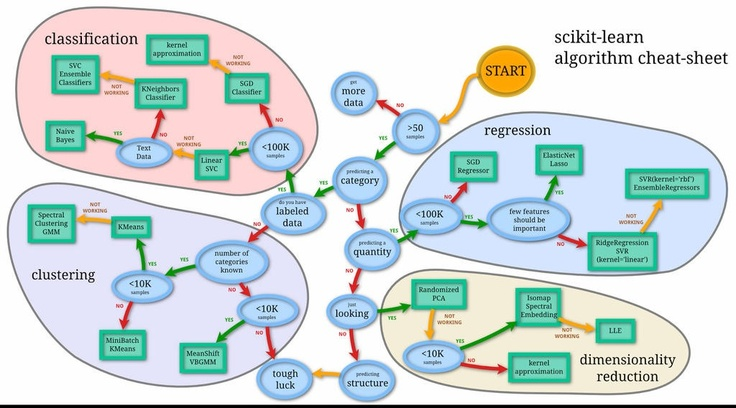
\includegraphics[width=0.8\linewidth,keepaspectratio]{SKLCheatSheet}
% \end{center}
% \end{frame}

% %%%%%%%%%%%%%%%%%%%%%%%%%%%%%%%%%%%%%%%%%%%%%%%%%%%%%%%%%%
% \begin{frame}[fragile]\frametitle{Cheat Sheet 2}
% \begin{center}
% 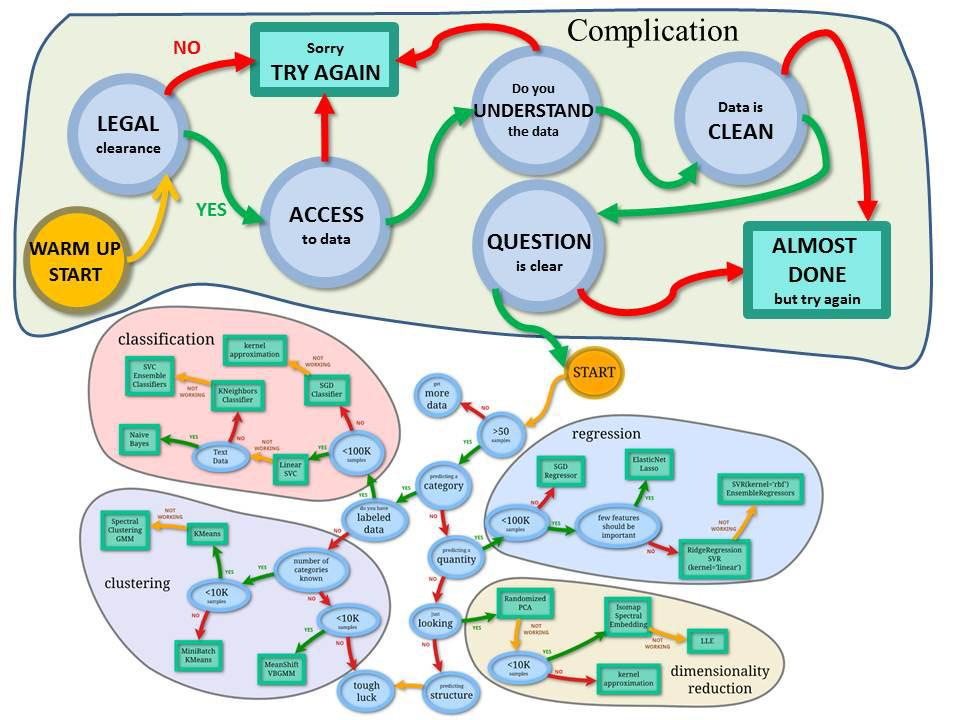
\includegraphics[width=0.8\linewidth,keepaspectratio]{SKLCheatSheet2}
% \end{center}
% \end{frame}

% %%%%%%%%%%%%%%%%%%%%%%%%%%%%%%%%%%%%%%%%%%%%%%%%%%%%%%%%%%%%%%%%%%%%%%%%%%%%%%%%%%
% \begin{frame}[fragile]\frametitle{}
% \begin{center}
% {\Large Sklearn: Algorithms}
% \end{center}
% \end{frame}

% %%%%%%%%%%%%%%%%%%%%%%%%%%%%%%%%%%%%%%%%%%%%%%%%%%%%%%%%%%
% \begin{frame}[fragile]\frametitle{Regression: Linear regression}
% \begin{lstlisting}
% from sklearn.linear_model import LinearRegression
% import matplotlib.pyplot as plt
% import numpy as np

% model = LinearRegression(normalize=True)

% x = np.arange(10)
% y = 2 * x + 1 + np.random.randn(10)
% plt.plot(x, y, 'o');
% plt.show()

% X = x[:, np.newaxis] # Making it 2D matrix

% model.fit(X, y)
% print(model.coef_)
% print(model.intercept_)

% xtest = np.array([1,23,10,14])
% XTest = xtest[:, np.newaxis]
% y_pred_test = model.predict(XTest)
% \end{lstlisting}
% \end{frame}


% %%%%%%%%%%%%%%%%%%%%%%%%%%%%%%%%%%%%%%%%%%%%%%%%%%%%%%%%%%%%%%%%%%%%%%%%
% \begin{frame}[fragile]\frametitle{Regression: Linear regression}
% Modify earlier program to have:
% \begin{itemize}
% \item \lstinline|x1 = np.arange(10)|
% \item \lstinline|x2 = np.arange(5,25,2)|
% \item \lstinline|y = 2*x1 + 4*x2 + 1 + np.random.randn(10) |
% \item \lstinline|X = np.column_stack((x1,x2)) |
% \item \lstinline|XTest = np.array([[2,3],[4,10],[3,20]]) |
% \item \lstinline|print(metrics.mean_squared_error(actual, predicted))|
% \item \lstinline|print(metrics.r2_score(actual, predicted))|
% \end{itemize}
% \end{frame}


% %
% %%%%%%%%%%%%%%%%%%%%%%%%%%%%%%%%%%%%%%%%%%%%%%%%%%%%%%%%%%%
% %\begin{frame}[fragile]\frametitle{Model}
% %\begin{lstlisting}
% %from sklearn import svm
% %
% %estimator = svm.SVC(gamma=0.001)
% %
% %estimator.fit(X, y)
% %
% %y_pred = estimator.predict(x)
% %
% %\end{lstlisting}
% %\end{frame}


% %%%%%%%%%%%%%%%%%%%%%%%%%%%%%%%%%%%%%%%%%%%%%%%%%%%%%%%%%%%
% %\begin{frame}[fragile]\frametitle{Classification: Linear regression}
% %\begin{lstlisting}
% %from sklearn import metrics
% %from sklearn import cross_validation as cv
% %
% %X_train, X_test, y_train, y_test     
% %	= cv.train_test_split(X, y, test_size=0.2)
% %
% %model      = ClassifierEstimator()
% %
% %model.fit(X_train, y_train)
% %
% %expected   = y_test
% %
% %predicted  = model.predict(X_test)
% %
% %print(metrics.classification_report(expected, predicted))
% %print(metrics.confusion_matrix(expected, predicted))
% %print(metrics.f1_score(expected, predicted))
% %\end{lstlisting}
% %\end{frame}
% %

% %%%%%%%%%%%%%%%%%%%%%%%%%%%%%%%%%%%%%%%%%%%%%%%%%%%%%%%%%%%
% %\begin{frame}[fragile]\frametitle{Coefficient of Determination}
% %\begin{lstlisting}
% %from sklearn import metrics
% %from sklearn import cross_validation as cv
% %
% %splits     = cv.train_test_split(X, y, test_size=0.2)
% %X_train, X_test, y_train, y_test = splits
% %
% %model      = RegressionEstimator()
% %
% %model.fit(X_train, y_train)
% %
% %expected   = y_test
% %
% %predicted  = model.predict(y_test)
% %
% %print(metrics.mean_squared_error(expected, predicted))
% %print(metrics.r2_score(expected, predicted))
% %\end{lstlisting}
% %\end{frame}

% %%%%%%%%%%%%%%%%%%%%%%%%%%%%%%%%%%%%%%%%%%%%%%%%%%%%%%%%%%%
% %\begin{frame}[fragile]\frametitle{Classification Example}
% %K nearest neighbors (kNN) is a supervised clustering/classification algorithm. Which group the unseen point belongs to, is classified.
% %\begin{lstlisting}
% %from sklearn import neighbors, datasets
% %
% %iris = datasets.load_iris()
% %X, y = iris.data, iris.target
% %
% %knn = neighbors.KNeighborsClassifier(n_neighbors=5)
% %
% %knn.fit(X, y)
% %
% %result = knn.predict([[3, 5, 4, 2],])
% %
% %print(iris.target_names[result])
% %
% %knn.predict_proba([[3, 5, 4, 2],])
% %\end{lstlisting}
% %\end{frame}
% %%%%%%%%%%%%%%%%%%%%%%%%%%%%%%%%%%%%%%%%%%%%%%%%%%%%%%%%%%
% \begin{frame}[fragile]\frametitle{Classifier: Support Vector Machine}

% \begin{lstlisting}
% from sklearn.svm import SVC

% model = SVC(kernel=``rbf'', C=1.0, gamma=1e-4)

% model.fit(X_train, y_train)

% predicted = model.predict(X_test)

% expected   = y_test

% from sklearn.metrics import f1_score

% print(f1_score(expected, predicted))
% \end{lstlisting}
% \end{frame}



% %%%%%%%%%%%%%%%%%%%%%%%%%%%%%%%%%%%%%%%%%%%%%%%%%%%%%%%%%%
% \begin{frame}[fragile]\frametitle{Classifier: K-Nearest neighbor classifier}
% For any unknown quantity, returns the label of the closest training point.

% \begin{lstlisting}
% from sklearn.neighbors import KNeighborsClassifier

% X, y = iris.data, iris.target

% clf = KNeighborsClassifier(n_neighbors=1)

% clf.fit(X, y)

% y_pred = clf.predict(X)

% print(np.all(y == y_pred))

% from sklearn.metrics import confusion_matrix

% print(confusion_matrix(y, y_pred))
% \end{lstlisting}
% \end{frame}



% %%%%%%%%%%%%%%%%%%%%%%%%%%%%%%%%%%%%%%%%%%%%%%%%%%%%%%%%%%
% \begin{frame}[fragile]\frametitle{Dimensionality Reduction: PCA}
% Principle Component Analysis (PCA) is a dimension reduction technique.
% \begin{lstlisting}
% X, y = iris.data, iris.target
% from sklearn.decomposition import PCA
% pca = PCA(n_components=2)
% pca.fit(X)
% X_reduced = pca.transform(X)
% print("Reduced dataset shape:", X_reduced.shape)

% \end{lstlisting}
% %
% %import pylab as pl
% %pl.scatter(X_reduced[:, 0], X_reduced[:, 1], c=y, cmap='RdYlBu')
% %
% %print("Meaning of the 2 components:")
% %for component in pca.components_:
% %    	print(" + ".join("%.3f x %s" % (value, name) for value, name in zip(component, iris.feature_names)))
% %    	
% \end{frame}

% %%%%%%%%%%%%%%%%%%%%%%%%%%%%%%%%%%%%%%%%%%%%%%%%%%%%%%%%%%
% \begin{frame}[fragile]\frametitle{Clustering: K-means}
% Clustering groups together observations that are homogeneous with respect to a given criterion.
% \begin{lstlisting}
% from sklearn.cluster import KMeans

% k_means = KMeans(n_clusters=3, random_state=0) 

% k_means.fit(X)

% y_pred = k_means.predict(X)

% pl.scatter(X_reduced[:, 0], X_reduced[:, 1], c=y_pred,
           % cmap='RdYlBu');
% \end{lstlisting}
% \end{frame}


% % %%%%%%%%%%%%%%%%%%%%%%%%%%%%%%%%%%%%%%%%%%%%%%%%%%%%%%%%%%%%%%%%%%%%%%%%%%%%%%%%%%
% % \begin{frame}[fragile]\frametitle{}
% % \begin{center}
% % {\Large Example Test Case}
% % \end{center}
% % \end{frame}


% % %%%%%%%%%%%%%%%%%%%%%%%%%%%%%%%%%%%%%%%%%%%%%%%%%%%%%%%%%%
% % \begin{frame}[fragile]\frametitle{Optical Character Recognition}
% % Loading and visualizing the digits data:
% % \begin{lstlisting}
% % from sklearn import datasets
% % import matplotlib.pyplot as plt

% % digits = datasets.load_digits()
% % print(digits.images.shape)

% % fig, axes = plt.subplots(10, 10, figsize=(8, 8))
% % fig.subplots_adjust(hspace=0.1, wspace=0.1)

% % for i, ax in enumerate(axes.flat):
    % % ax.imshow(digits.images[i], cmap='binary')
    % % ax.text(0.05, 0.05, str(digits.target[i]),
            % % transform=ax.transAxes, color='green')
    % % ax.set_xticks([])
    % % ax.set_yticks([])

% % plt.show()
% % \end{lstlisting}
% % \end{frame}


% % %%%%%%%%%%%%%%%%%%%%%%%%%%%%%%%%%%%%%%%%%%%%%%%%%%%%%%%%%%
% % \begin{frame}[fragile]\frametitle{Inputs}
% % Here the data is simply each pixel value within an 8x8 grid:
% % \begin{lstlisting}
% % print(digits.images.shape)
% % print(digits.images[0])

% % (1797, 8, 8)
% % [[  0.   0.   5.  13.   9.   1.   0.   0.]
 % % [  0.   0.  13.  15.  10.  15.   5.   0.]
 % % [  0.   3.  15.   2.   0.  11.   8.   0.]
 % % [  0.   4.  12.   0.   0.   8.   8.   0.]
 % % [  0.   5.   8.   0.   0.   9.   8.   0.]
 % % [  0.   4.  11.   0.   1.  12.   7.   0.]
 % % [  0.   2.  14.   5.  10.  12.   0.   0.]
 % % [  0.   0.   6.  13.  10.   0.   0.   0.]]

% % \end{lstlisting}
% % So our data have 1797 samples in 64 dimensions.
% % \end{frame}
% % %
% % %%%%%%%%%%%%%%%%%%%%%%%%%%%%%%%%%%%%%%%%%%%%%%%%%%%%%%%%%%%
% % %\begin{frame}[fragile]\frametitle{Unsupervised Learning: Dimensionality Reduction}
% % %We'd like to visualize our points within the 64-dimensional parameter space, but it's difficult to plot points in 64 dimensions! Instead we'll reduce the dimensions to 2, using an unsupervised method. Here, we'll make use of a manifold learning algorithm called Isomap, and transform the data to two dimensions.
% % %\begin{lstlisting}
% % %from sklearn.manifold import Isomap
% % %
% % %iso = Isomap(n_components=2)
% % %
% % %data_projected = iso.fit_transform(digits.data)
% % %
% % %print(data_projected.shape)
% % %
% % %plt.scatter(data_projected[:, 0], data_projected[:, 1], c=digits.target,
% % %            edgecolor='none', alpha=0.5, cmap=plt.cm.get_cmap('nipy_spectral', 10));
% % %plt.colorbar(label='digit label', ticks=range(10))
% % %plt.clim(-0.5, 9.5)
% % %\end{lstlisting}
% % %
% % %\end{frame}


% % %%%%%%%%%%%%%%%%%%%%%%%%%%%%%%%%%%%%%%%%%%%%%%%%%%%%%%%%%%
% % \begin{frame}[fragile]\frametitle{Classification on Digits}
% % The first thing we'll want to do is split the digits into a training and testing sample:
% % \begin{lstlisting}
% % from sklearn.cross_validation import train_test_split

% % Xtrain, Xtest, ytrain, ytest = train_test_split(digits.data, digits.target,random_state=2)

% % print(Xtrain.shape, Xtest.shape)

% % from sklearn.linear_model import LogisticRegression

% % clf = LogisticRegression(penalty='l2')

% % clf.fit(Xtrain, ytrain)

% % ypred = clf.predict(Xtest)

% % from sklearn.metrics import accuracy_score
% % accuracy_score(ytest, ypred)

% % \end{lstlisting}

% % \end{frame}

% %%%%%%%%%%%%%%%%%%%%%%%%%%%%%%%%%%%%%%%%%%%%%%%%%%%%%%%%%%
% \begin{frame}[fragile]\frametitle{Results}
% \begin{lstlisting}
% plt.imshow(np.log(confusion_matrix(ytest, ypred)),
          % cmap='Blues', interpolation='nearest')
% plt.grid(False)
% plt.ylabel('true')
% plt.xlabel('predicted');
% \end{lstlisting}
% \begin{center}
% 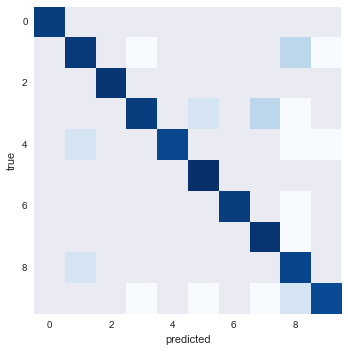
\includegraphics[width=0.5\linewidth,keepaspectratio]{optresult}
% \end{center}
% \end{frame}

